\chapter{Background \& State of the art}
\label{chapter:sota}

This chapter discusses the state of the art in the areas of \emph{\wasm} and \emph{Software Diversification}. In \autoref{sota:wasm} we discuss the \wasm language, its motivation, how \wasm binaries are generated, the language specification, and security-related issues. In \autoref{sota:sota}, we present a summary of Software Diversification, its foundational concepts and highlighted related works.  
We select the discussed works by their novelty, critical insights, and representativeness of their techniques. 
In \autoref{sota:openchallenges}, we finalize the chapter by highlighting open challenges in state-of-the-art related works.


%In \autoref{sota:wasm} we describe the context in which this dissertation is based, \wasm. We include both usage scenarios for Wasm and its main security issues. In \autoref{sota:diversification} we discuss the main diversification techniques in the wild, we introduce the concept of superoptimization used in this work, and we end the section by highlighting superdiversification as the cornerstone of our contributions are based. In \autoref{sota:randomization} we mention close works to runtime diversification and how diversification can be used to construct resilient binaries. 

\section{\wasm\ overview}
\label{sota:wasm}

%\renewcommand{\lstnumberautorefname}{Line}
\newcommand{\lstnumberautorefname}{Line}
\newcommand{\lineref}[1]{\autoref{#1}}


%\todo{Intro}

%\subsection*{}

% Javascript was first, and then more attempts.
JavaScript is currently used in all modern web browsers to allow client-side scripting. However, due to the complexity of this language, its security flaws and to gain in performance, several alternatives appeared through the years.  For example, Java applets were introduced on web pages late in the 90s to execute Java bytecode in the client side \cite{javaapplet}. Similarly, Microsoft made two attempts with ActiveX in 1996 \cite{activex}, and with Silverlight in 2007 \cite{silverlight}. All these attempts failed to persist or had low adoption, mainly due to security issues and the lack of consensus on the community of browser vendors.

% asm.js and the demonstration of bad language patterns
In 2014, Alon Zakai and colleagues proposed the Emscripten tool \cite{emscripten}. Emscripten used a strict subset of JavaScript, asm.js, to allow low-level code such as C to be compiled to JavaScript. Asm.js was first announced as an LLVM backend \cite{asmjsweb}. This approach came with the benefits of having all the ahead-of-time optimizations from LLVM, gaining in performance on browser clients \cite{asmjs} compared to standard JavaScript code. Asm.js was faster than JavaScript because it limited the language features to those that can be optimized in the LLVM pipeline. Besides, it removed the majority of the dynamic characteristics of the language, limiting it to numerical types, top-level functions, and one large array in the memory directly accessed as raw data. Since asm.js was a subset of JavaScript it was compatible with all engines at that moment. Asm.js demonstrated that client-code could be improved with the right language design and standardization.
% Limitations o0f asm.js and the birth of Wasm
The work of Van Es \etal \cite{EsAsm.js} proposed to shrink JavaScript to asm.js in a source-to-source strategy, closing the cycle and extending the fact that asm.js was mainly a compilation target for C/C++ code. 
%
Nevertheless, JavaScript faces several limitations related to the characteristics of the language. For example, any JavaScript engine requires the parsing and recompiling the JavaScript code which implies a significant overhead.


Following the asm.js initiative, the W3C publicly announced the \wasm\ (Wasm) language in 2017. \wasm\ is a binary instruction format for a stack-based virtual machine and was officially consolidated by the work of Haas \etal \cite{Haas_2017} in 2017. The announcement of \wasm\ marked the first step into the standardization of bytecode in the web environment. Wasm  is designed to be fast, portable, self-contained and secure, and it outperforms asm.js \cite{Haas_2017}. Since 2017, the adoption of \wasm\ keeps growing. For example; Adobe, announced a full online version of Photoshop\footnote{\url{https://twitter.com/Adobe/status/1453034805004685313?s=20&t=Zf1N7-WmzecA0K4V8R69lw}} written in WebAssembly;  game companies moved their development from JavaScript to Wasm like is the case of a full Minecraft version\footnote{\url{https://satoshinm.github.io/NetCraft/}}; and the case of Blazor\footnote{\url{https://dotnet.microsoft.com/en-us/apps/aspnet/web-apps/blazor}}, a .Net virtual machine implemented in Wasm, able to execute C\# code in the browser.

%\todo{Benchmarks}

\subsection{From source to Wasm}

All \wasm\ programs are compiled ahead-of-time from source languages. LLVM includes Wasm  as a backend since release 7.1.0 published in May 2019\footnote{\url{https://github.com/llvm/llvm-project/releases/tag/llvmorg-7.1.0}}, supporting a broad range of frontend languages such as C/C++, Rust, Go or AssemblyScript\footnote{subset of the TypeScript language}. The resulting binary works similarly to a traditional shared library, it includes instruction codes, symbols and exported functions. In \autoref{diagrams:sota:wasm}, we illustrate the workflow from the creation of Wasm  binaries to their execution in the browser. The process starts by compiling the source code program to Wasm  (Step \step{1}). This step includes ahead-of-time optimizations such as optimizations in the LLVM toolchain. 

%To the best of our knowledge, the most complete survey about Wasm  tooling is presented in the Awesome Wasm  (\url{https://github.com/mbasso/awesome-wasm}) repo. It is a cumulative GitHub repo which includes references to articles, papers, books, demos, compilers and engines related to \wasm. 

The step \step{2} builds the standard library for Wasm  usually as JavaScript  code. This code includes the external functions that the Wasm  binary needs for its execution inside the host engine. For example, the functions to interact with the DOM of the HTML page are imported in the Wasm  binary during its call from the JavaScript code. The standard library can be manually written, however, compilers like Emscripten, Rust and Binaryen can generate it automatically, making this process completely transparent to developers.

Finally, the third step (Step \step{3}), includes the compilation and execution of the client-side code. Most of the browser engines compile both the Wasm  and JavaScript codes to machine code. In the case of JavaScript, this process involves JIT and hot code replacement during runtime. For Wasm, since it is closer to machine code, and it is already optimized, this process is a one-to-one mapping. For instance, in the case of V8, the compilation process only applies simple and fast optimizations such as constant folding and dead code removal. Once V8 completes the compilation process, the generated machine code for Wasm does not change anymore and is the same used along all its executions. This analysis was validated by conversations with the V8's development team and by experimental studies in one of our contributions \cite{CROW}.  

\begin{figure}[h]
    \centering
    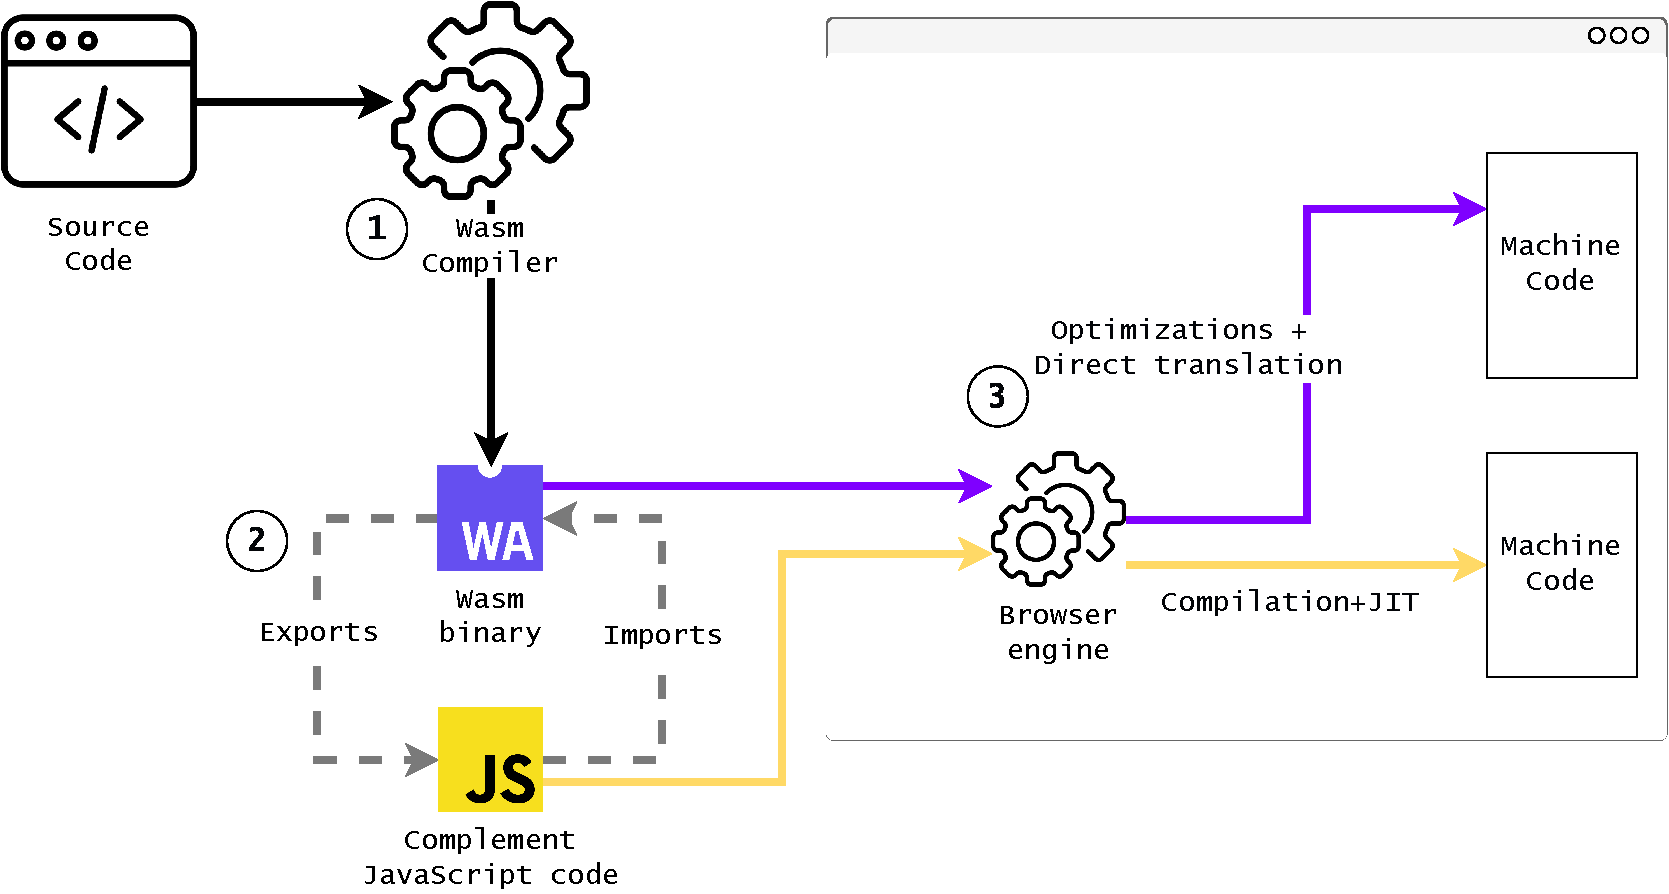
\includegraphics[width=\linewidth]{diagrams/wasm_workflow.pdf}
    \caption{WebAssembly is built, then compiled by the host web browser and finally executed. }
    \label{diagrams:sota:wasm}
\end{figure}

Wasm can execute directly and is platform independent.
Thus, the Internet of Things (IoT) can be seen as the perfect match for \wasm\ \cite{Narayan2021Swivel,Sledge} outside web browsers.
IoT devices are heterogeneous in terms of architecture and platform as the same for Edge computing.
For example, Singh and colleagues \cite{WARDuino2019} proposed a virtual machine for Wasm in arduino based devices.
On the other hand, Cloudflare and Fastly adapted their platforms to provide edge computing services directly with \wasm. 
In these cases, the standard library, instead of JavaScript, is provided by any other language stack that the host environment supports.

In 2019, the Bytecode Alliance \cite{bytecodealliance} proposed the WebAssembly System Interface (WASI) \cite{WASI}. 
WASI is the foundation to build Wasm code outside the browser with a POSIX system interface platform. 
WASI standardizes the adoption of \wasm\ in heterogeneous platforms \cite{bryant2020webassembly}. 

% Talk about benchmarks and performance numbers

%

%\todo{How to obtain WebAssemblybinaries}

%\todo{Browser workflow}

%\todo{How interpreters work, explain the workflow of V8 as it was validated by the V8 compiler developers}

%\todo{Backend workflow}

%\todo{Add a table with tools and interpreters: V8, SpiderMonkey, wasmtime, wasmer, sledge, warduino }


\subsection{WebAssembly specification}

% General description and the introduction of the component, module and section terms
\wasm\ defines its own Instruction Set Architecture (ISA) \cite{wasm_spec}. It is an abstraction close to machine code instructions but agnostic to CPU architectures. Thus, Wasm  is platform independent. The ISA of Wasm  includes also the necessary components that the binary requires to run in any host engine. 
A Wasm  binary has a unique module as its main component. A module is composed by sections, corresponding to 13 types\footnote{\url{https://webassembly.github.io/spec/core/binary/modules.html\#sections}}, each of them with an explicit semantic and a specific order inside the module. This makes the compilation to machine code faster. %The binary format of Wasm  can include custom sections. For example, the work of \todo{Doe} proposed the usage of custom sections to sign binaries for the sake of trusting. 


% Example and intro to the stack
In \autoref{CExample} and \autoref{WASMExample} we illustrate a C program and the Wasm program that results from its compilation. The C function contains: heap allocation, external function declaration and the definition of a function with a loop, conditional branching, function calls and memory accesses. The code in \autoref{WASMExample} shows the textual format for the generated Wasm. The module in this case first defines the signature of the functions (\lineref{tpe1}, \lineref{tpe2}  and  \lineref{tpe3})  that help in the validation of the binary defining its parameter and result types. The information exchange between the host and the Wasm  binary might be in two ways, exporting and importing functions, memory and globals to and from the host engine (\lineref{import1}, \lineref{export1} and \lineref{export2}). The definition of the function (\lineref{func1}) and its body follows the last import declaration at \lineref{import1}. 

% Functions
The function body is composed of local-variable declarations and typed instructions that are evaluated using a virtual stack (Line 7 to Line 32 in \autoref{WASMExample}). Each instruction reads its operands from the stack and pushes back the result. The result of a function call is the top value of the stack at the end of the execution. In the case of \autoref{WASMExample}, the result value of the main function is the calculation of the last instruction, \texttt{i32.add} at \lineref{result}. A valid Wasm  binary should have a valid stack structure that is verified during its translation to machine code. The stack validation is carried out using the static types of Wasm, \texttt{i32} for 32 bits signed integer, \texttt{i64} for 64 bits signed integer, \texttt{f32} for 32 bits float and \texttt{f64} for 64 bits float. As the listing shows, instructions are annotated with a numeric type.

% Example
\begin{code}
    \begin{minipage}[t]{0.45\linewidth}
        \lstset{language=C,caption={Example C function.},
        label=CExample,
        breaklines=true, 
        basicstyle=\small\ttfamily,
        postbreak=\mbox{\textcolor{red}{$\hookrightarrow$}\space},
        escapeinside={(*@}{@*)}
        }
\input{sota/code/code.c}
\end{minipage}\hspace{10mm}
\begin{minipage}[t]{0.46\linewidth}
\lstset{
    language=WAT,
    caption={\wasm\ code  for \autoref{CExample}.},
    style=WATStyle,
    breaklines=true, 
    %stepnumber=0,
    escapeinside={(*@}{@*)},
    numbers=left,
    postbreak=\mbox{\textcolor{red}{$\hookrightarrow$}\space},
    label=WASMExample}
%
\input{sota/code/code.fix.wat}
%\end{lstlisting}
\end{minipage}


%\begin{tikzpicture}[remember picture,overlay]

%\path (2.west) edge[<-, black] (1.west);
%\path (3.west) edge[<-,  black] (4.west);

%\path (6.east) edge[<-, bend right, black] (3.east);
%\path (9.east) edge[<-, bend right, black] (4.east);
%\path (7.east) edge[<-, bend right, black] (8.east);


%\end{tikzpicture}
\end{code}

% Memory, globals and functions
Wasm  manages the memory in a restricted way. A Wasm  module has a linear memory component that is accessed with \texttt{i32} pointers (integer of 32 bits) and should be isolated from the virtual stack. The declaration of the linear data in the memory is showed in \lineref{data}. The memory access is illustrated in \lineref{load}. This memory is usually bound in browser engines to 4Gb of size, and it is only shareable between the process that instantiate the Wasm  binary and the binary itself (explicitly declared in \lineref{mem1} and \lineref{export2}). This ensures the isolation of the execution of Wasm  code. 

Wasm  also provides global variables in their four primitive types. Global variables (\lineref{global1}) are only accessible by their declaration index, and it is not possible to dynamically address them. For functions, Wasm  follows the same mechanism, either the functions are called by their index (\lineref{call}) or using a static table of function declarations. The latter allows modeling dynamic calls of functions (through pointers) from languages such as C/C++, for which the Wasm's compiler is in charge of populating the static table of functions.


In Wasm, all instructions are grouped into blocks, where the start of a function is the root block. Two consecutive block declarations can be appreciated in \lineref{block1} and \lineref{block2} of \autoref{WASMExample}. Control flow structures jump between block boundaries and not to any position in the code like regular assembly code. A block may specify the state that the stack must have before its execution and the result stack value coming from its instructions. Inside the Wasm  binary the blocks explicitly define where they start and end (\lineref{end1} and \lineref{end2}). By design, each block executes independently and cannot execute or refer to outer block codes. This is guaranteed by explicitly annotating the state of the stack before and after the block. Three instructions handle the navigation between blocks: unconditional break, conditional break (\lineref{break1} and \lineref{break2}) and table break. Each break instruction can only jump to one of its enclosing blocks. For example, in \autoref{WASMExample}, \lineref{break1} forces the execution to jump to the end of the first block that starts at \lineref{block1} if the value at the top of the stack is greater than zero.

%We want to remark that de description of Wasm  in this section follows the version 1.0 of the language and not its proposals for extended features. We follow those features implemented in the majority of the vendors according to the Wasm roadmap \cite{wasm_roadmap}. On the other hand we excluded instructions for datatype conversion, table accesses and the majority of the arithmetic instructions for the sake of simplicity.

%There are two types of blocks, regular blocks, used to compound pieces of code for stack validation and loops. A loop block manages iterations, the only difference between this to blocks is that the breaking instruction jumps to the end of the block in the case of loops.

% Self contained loops

% Bound memory, no direct access to the DOM

% Roadmap: threads, SIMD, etc

%\todo{Wasm  Semantics: Add a code listing, explain General layout of a binary, Function and signature, Instructions, Control flow, Memory model, Global model, table model}

%\todo{Add some sentences from the roadmap}

%\todo{Exported function signature allows typing validation before the code is executed}


\subsection{WebAssembly security}

As we described, \wasm\ is deterministic and well-typed, follows a structured control flow and explicitly separates its linear memory model, global variables and the execution stack. This design is robust \cite{WebAssemblySecurity} and makes it easy for compilers and engines to sandbox the execution of Wasm  binaries. Following the specification of Wasm  for typing, memory, virtual stack and function calling,
host environments should provide protection against data corruption, code injection, and return-oriented programming (ROP).

However, implementations in both browsers and standalone runtimes~\cite{Narayan2021Swivel} are vulnerable.
Genkin \etal demonstrated that Wasm  could be used to exfiltrate data using cache timing-side channels \cite{Genkin2018DrivebyKC}.
Moreover, binaries itself can be vulnerable. The work of Lehmann \etal ~\cite{usenixWasm2020} proved that C/C++ source code vulnerabilities can propagate to Wasm  such as overwriting constant data or manipulating the heap by overflowing the stack. Even though these vulnerabilities need a specific standard library implementation to be exploited, they make a call for better defenses for \wasm. 
Recently, Stiévenart and colleagues demonstrate that C/C++ source code vulnerabilities can be ported to Wasm \cite{DeRoover2022}.
% Current proposals
Several proposals for extending \wasm\ in the current roadmap could address some existing vulnerabilities. For example, having multiple memories\footnote{\url{https://github.com/WebAssembly/multi-memory/blob/main/proposals/multi-memory/Overview.md}} could incorporate more than one memory, stack and global spaces, shrinking the attack surface. However, the implementation, adoption and settlement of the proposals are far from being a reality in all browser vendors\footnote{\url{https://webassembly.org/roadmap/}}. 
% In fact, according to the work of Hilbig \etal \cite{Hilbig2021AnES}, the artificial variants created with one of our works contribute to the half of executable and available \wasm\ binaries in the wild.


\section{Software Diversification}
\label{sota:sota}
%Checkmarck symbol
\def\checkmark{\tikz\fill[scale=0.4](0,.35) -- (.25,0) -- (1,.7) -- (.25,.15) -- cycle;} 

% Commands to refer to the milestones
\newtheoremstyle{sota}% name of the style to be used
  {\topsep}% measure of space to leave above the theorem. E.g.: 3pt
  {\topsep}% measure of space to leave below the theorem. E.g.: 3pt
  {\itshape}% name of font to use in the body of the theorem
  {0pt}% measure of space to indent
  {\bfseries}% name of head font
  {}% punctuation between head and body
  { }% space after theorem head; " " = normal interword space
  {(\thmname{#1}\thmnumber{#2})\textnormal{\thmnote{ (#3)}}}

\def\Gnospace~{G{}}
\theoremstyle{sota}
\newtheorem{goal}{G}
\providecommand*{\definitionautorefname}{\Gnospace}
\newcommand{\goalautorefname}{\Gnospace}


\def\Snospace~{S{}}
\theoremstyle{sota}
\newtheorem{strategy}{S}
\providecommand*{\definitionautorefname}{\Snospace}
\newcommand{\strategyautorefname}{\Snospace}

\def\Unospace~{U{}}
\theoremstyle{sota}
\newtheorem{usage}{U}
\providecommand*{\definitionautorefname}{\Unospace}
\newcommand{\usageautorefname}{\Unospace}

%\%todo{Esta muy regado ahora.}

%\todo{Stress input-output equivalence in the artificial diversification.}

%\todo{Mention concrete objective and achievement when citing.}

%\todo{emove some strategies, just cite some papers and thats it. Reduce to five transformations. Stick to U2 andd U3. Add techincal stack in the table.}

%\todo{Add level of transformation as a dimension. Hoigh level, fine-grained transofmrations, etc}

%\todo{Start with COhen, then go form high level to fine granied and from technologies to LLVM and Wasm.}


%\todo{Given a collection of pgorams, then enumerate the usages. Second approach, multiple encapsulation in one single program.}

Software Diversification has been widely studied in the past decades. This section discusses its state of the art.
% What is Software diversity
Software diversification consists in synthesizing, reusing, distributing, and executing different, functionally equivalent programs. 
According to the survey of Baudry and Monperrus \cite{natural_diversity}, the motivation for software diversification can be separated in five categories: reusability \cite{pohl2005software}, software testing \cite{Chen2010AdaptiveRT}, performance \cite{10.1145/2025113.2025133}, fault tolerance \cite{1659219} and security \cite{cohen1993operating}. Our work contributes to the latter two categories. In this section we discuss related works by highlighting how they generate diversification and how they use the generated diversification. We finalize by comparing our contributions with the related work.

\subsection*{Artificial Software Diversity.}

There are two primary sources of software diversification: Natural and Artificial Diversity \cite{natural_diversity}. This work contributes to the state of the art of Artificial Diversity, which consists of artificially synthesizing software. 
% Intro to Cohen and that functional/semantic equivalence is 
We have found that the foundation for automatic software diversity has barely changed since Cohen in 1993 \cite{cohen1993operating}. Therefore, the work of Cohen is the cornerstone of this dissertation.
According to their seminal work, whatever two programs are equal if they are semantically equivalent, thus, one program can be considered a diversified version of the other. 
They defined semantic/functional equivalence as input-output equivalence. Two programs are equivalent if, given identical input, they produce the identical output. 

% Mutation strategy
Cohen \etal proposed to generate automatic software diversification through mutation strategies.
A mutation strategy is a set of rules to define how a specific component of software development should be changed to provide a different yet functionally equivalent program. Cohen \etal proposed 10 concrete transformation strategies that we summarize, complemented with the work of Baudry and Monperrus \cite{natural_diversity} and the work of Jackson \etal \cite{jackson}, in 5 strategies.

% A mutation can be applied at different layers of software lifecycle, from compilation to execution and from source code to executable binary.


%Natural diversity can be controlled or an unpredicted consequence of developing processes. Controlled natural diversity is usually called Design Diversity or N-Version Diversity. It is addressed using engineering decisions \cite{1659219}. 
%In practice, Natural Diversity consists of providing N development teams with the exact requirements. The teams develop N independent versions using different approaches. On the other hand, Natural Diversity can emerge from spontaneous software development processes. To illustrate the Natural Diversity phenomenon, CodeForces\footnote{\url{https://codeforces.com/contest/1667/status/page/2?order=BY_PROGRAM_LENGTH_ASC}} shows more than 350 different and successful solutions in C++ for a single requirements based problem in a single programming contest. 
%The software market is an expected source of natural diversity. Sengupta \etal \cite{10.5555/3091125.3091155} used this fact to reach the security goal (\autoref{goal:security}).



% Jump to the need of artificial
%Notice that Natural Diversity can rely on itself to escalate, and it is coped by the preexistence of software. This might be a limitation. For example, in the context o this work, the natural diversity for \wasm programs is nearly inexistence \cite{Hilbig2021AnES}. When natural diversity is not enough, it is innate to think that the source for diversification needs to be artificial. 

% Classification by Cohen



\begin{strategy}{Equivalent instructions replacement}
    \label{strategy:S1}
    \normalfont 
    Pieces of programs can be replaced by semantically equivalent code such as equivalent arithmetic expressions, including the adding of garbage instructions, \ie instructions that do not affect the computation result. This strategy is simple but powerful since the complexity of program variants dramatically increases. In terms of overhead, the size of the program variant increases with the size of the replacement. Usually, the replacement rules are written by hand as code templates representing a piece of code and a valid replacement for it, similar to compiler optimization rules. For example, Jackson \etal \cite{jackson2011compiler} highlighted the usage of  the optimization flags of several compilers to generate semantically equivalent binaries. On the same topic, Cleemput \etal \cite{Cleemput2012} and Homescu \etal~\cite{homescu2013profile} introduce the usage of inserting NOP instructions to generate statically different variants at each compilation. 


    %Jackson \etal \cite{jackson} have explored how to use NOP operations inserted during compiling time to diversify programs \todo{which stack, if LLVM merge with the previous one}. 
    % However, this approach is limited by the number of available flags in the compiler implementation and because the optimization is applied in all possible places in the code at the same time.
    Exhaustive exploration is another approach to generate equivalent instructions. This technique is based on sampling or constructing all possible programs for a specific language. Once a program is found, it is checked for semantically equivalence against the original program, reporting it as a variant if is the case.
     Jacob \etal \cite{jacob2008superdiversifier} proposed the technique called superdiversification for x86 binaries. They generate semantically equivalent transformations at basic block level that outperform transformations written by human experts. Similarly, Tsoupidi \etal \cite{Tsoupidi2020ConstraintBasedSD} introduced Diversity by Construction, a constraint-based compiler to generate software diversity for MIPS32 architecture. Their technique relies in using a constraint solver to generate program variants that by construction are semantically equivalent. Compared to other techniques, the works of Jacob \etal and Tsoupidi \etal do not need the writing of transformation strategies by hand, but they are limited by the reach of theorem solvers and can only be applied statically. 
     \\
     \\

    %An enumerative synthesis is a brute-force approach to generate program variants. With a maximum number of instructions, it constructs and checks all possible programs up to that limit. For a simplified instance, with a maximum code size of 2 instructions in a programming language with $L$ possible constructions, an enumerative synthesizer builds and checks all $L\times L$ combinations of programs. 
    %
\end{strategy}


\begin{strategy}{Instruction reordering}
    \label{strategy:S2}
    \normalfont
    This strategy reorders instructions or entire program blocks if they are independent.
    The location of variable declarations might change as well if compilers resort them in the symbol tables. It prevents static examination and analysis of parameters and alters memory locations. The strategy should not affect the size of program variants neither their execution time. For example, Bhatkar \etal \cite{bhatkar03, bhatkar2005efficient} proposed the random permutation of the order of variables and routines for ELF binaries.
\end{strategy}

\begin{strategy}{Adding, changing, removing jumps and calls}
    \label{strategy:S3}
    \normalfont
    This strategy creates program variants by adding, changing, or removing jumps and calls in the original program. Cohen \cite{cohen1993operating} mainly illustrated the case by inserting bogus jumps in programs. Pettis and Hansen \cite{pettisochhansen} proposed to split basic blocks and functions for the PA-RISC architecture, inserting jumps between splits.
    Similarly, Crane \etal~\cite{crane2015thwarting} de-inline basic blocks of code as an LLVM 3.3 pass. In their approach, each de-inlined code is transformed into semantically equivalent functions that are randomly selected at runtime to replace the original code calculation. On the same topic, Bhatkar \etal \cite{bhatkar2005efficient} extended their previous approach \cite{bhatkar03}, replacing function calls by indirect pointer calls in C source code, allowing post binary reordering of function calls.
\end{strategy}


\begin{strategy}{Program memory and stack randomization}
    \label{strategy:S4}
    \normalfont
    This strategy changes the layout of programs in the host memory. Also, it can randomize how a program variant operates its memory. The work of Bhatkar \etal \cite{bhatkar03, bhatkar2005efficient} also proposed to randomize the base addresses of applications and the library memory regions, and the random introduction of gaps between memory objects in ELF binaries. Tadesse Aga and Autin \cite{aga2019smokestack} and Lee \etal \cite{lee2021savior} recently proposed a technique to randomize the local stack organization for function calls using a custom LLVM compiler.
    Younan \etal \cite{Younan2006} proposed to separate a conventional stack into multiple stacks where each stack contains a particular class of
    data. 
    On the same topic, Xu \etal \cite{xu2020merr} transform programs to reduce memory exposure time, improving the time needed for frequent memory address randomization. 
    %This makes it very hard for an attacker to ignore the key to inject executable code. This breaks the predictability of program execution and mitigates certain exploits. 
\end{strategy}


\begin{strategy}{ISA randomization and simulation}
    \label{strategy:S5}
    \normalfont
    This strategy encodes the original program binary. Once encoded, the program can be decoded only once at the target client, or it can be interpreted in the encoded form using a custom virtual machine implementation. This technique is strong against attacks involving the examination of code. It does not affect the size of program variants or their execution times.
    Kc \etal and Barrantes \etal \cite{Kc03,barrantes2003randomized} proposed seminal works on instruction-set randomization 
    to create a unique mapping between artificial CPU instructions and real ones.
    On the same topic, Chew, and Song \cite{Chew02mitigatingbuffer} target operating system randomization. They randomize the interface between the operating system and the user applications.
    Courouss{\'e} \etal~\cite{courousse2016runtime} implement an assembly-like DSL to generate equivalent code at runtime in order to increase protection against side-channel attacks. Their technique generates a different program during execution using an interpreter for their DSL.

    %It is an interpretation mechanism similar to encoding (\autoref{strategy:S9}), but the execution of programs is delegated to a custom interpreter instead of using preexisting execution hosts. The program is decoded at runtime every time it is invoked. 
    
\end{strategy}


\begin{comment}

\begin{strategy}{Intermixing}
    \label{strategy:S10}
    \normalfont
    With the existence of more than one program variant, the execution of program variants can be mixed. The decision of which variant executes is decided at runtime. This strategy is the core for randomization, multivariant execution and the execution by consensus defined in \autoref{goal:reliability}. This strategy is 
    complex to implement because the integrity of the memory and stack needs to be stable between programs.
\end{strategy}
\end{comment}

%\subsection*{Vertical Software Diversification}

The mentioned techniques can be applied at any layer of the software lifecycle, at coarse-grained or fine-grained levels.
At high-level, Harrand \etal, propose to merge several Java decompiler variants to provide an extended and improved meta-decompiler \cite{harrand2020java}. On the same topic, Sengupta \etal \cite{10.5555/3091125.3091155} shift several database engines and backends for web applications. Their idea makes known CVEs to be available only in certain time window, making potential attackers to not always success. Moreover, Roi \etal \cite{10.1145/3318216.3363338} proposed to use several machine learning algorithms with the same task to tackle adversarial attackers, using a different algorithm every time the system was queried.
These works used preexisting software diversity to provide improved systems, both for reliability and security.

For fine-grained diversification, the before mentioned mutation strategies can be applied directly to the basecode at the instruction level, during the compilation of programs or directly to the generated binaries. As we previously mentioned Homescu \etal \cite{homescu2013profile}, Jackson \etal \cite{jackson, jackson2011compiler}, Jacob \etal \cite{jacob2008superdiversifier}, Crane \etal \cite{crane2015thwarting}, Aga \etal \cite{aga2019smokestack} \todo{add all the others} and Tsoupidi \etal \cite{Tsoupidi2020ConstraintBasedSD} placed compilers in their diversification techniques. Similarly, Bathkar \etal \cite{bhatkar03,bhatkar2005efficient}, Chew and Song \cite{Chew02mitigatingbuffer}, El-Khalil and Keromytis \cite{ElKhalil2004}, and Cohen \cite{cohen1993operating} itself mostly proposed binary to binary transformations. 
We have observed that fine-grained techniques are mainly motivated because they provide more robust diversification in terms of preservation. For example, to apply diversification techniques closer to the final execution avoid removing of code transformations by later optimization or compilation stages. Our contributions are fine-grained based. 

%Superdiversifier, all the others, and then finish with that we contribute to fine-grained.

\subsection*{Usages of Software Diversity}

After program variants are generated, they can be used in two main scenarios: Randomization or Multivariant Execution(MVE) \cite{jackson}. In \autoref{diagrams:sota:randomization} and \autoref{diagrams:sota:mve} we illustrate both scenarios. 



\newcommand{\rulesep}{\unskip\ \vrule\ }
\begin{figure}[h]
    \centering
    \begin{subfigure}[t]{0.45\textwidth}
        \centering
        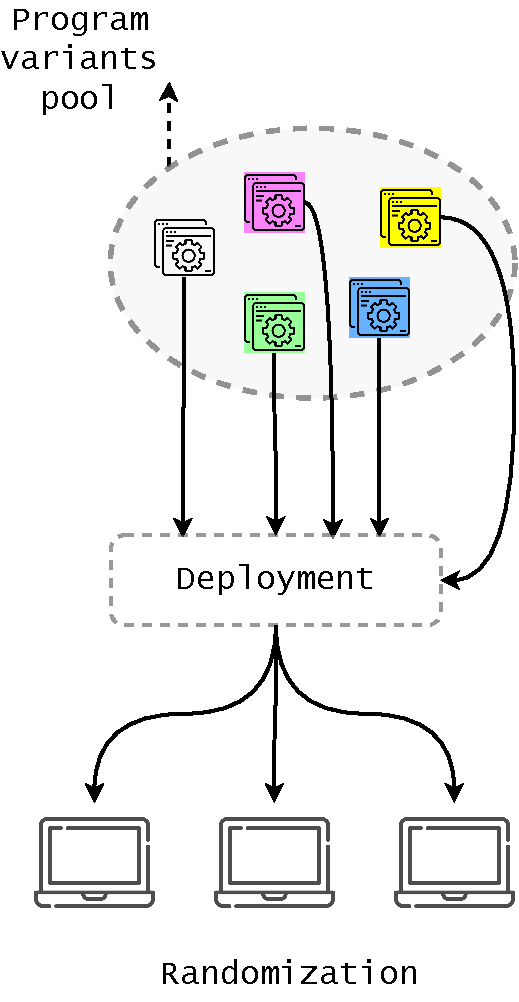
\includegraphics[height=3.1in]{diagrams/randomization.pdf}
        \vspace{0.5cm}
        \caption{Randomization scenario. Given a pool of program variants, one variant is deployed per host. Each deployment randomly selects which variant is assigned to each host. The same program variant is executed in the host at every program invocation between deployments. }        \label{diagrams:sota:randomization}

    \end{subfigure}
    \hspace{1.5mm}
    \rulesep
    \hspace{1.5mm}
    \begin{subfigure}[t]{0.45\textwidth}
        \centering
        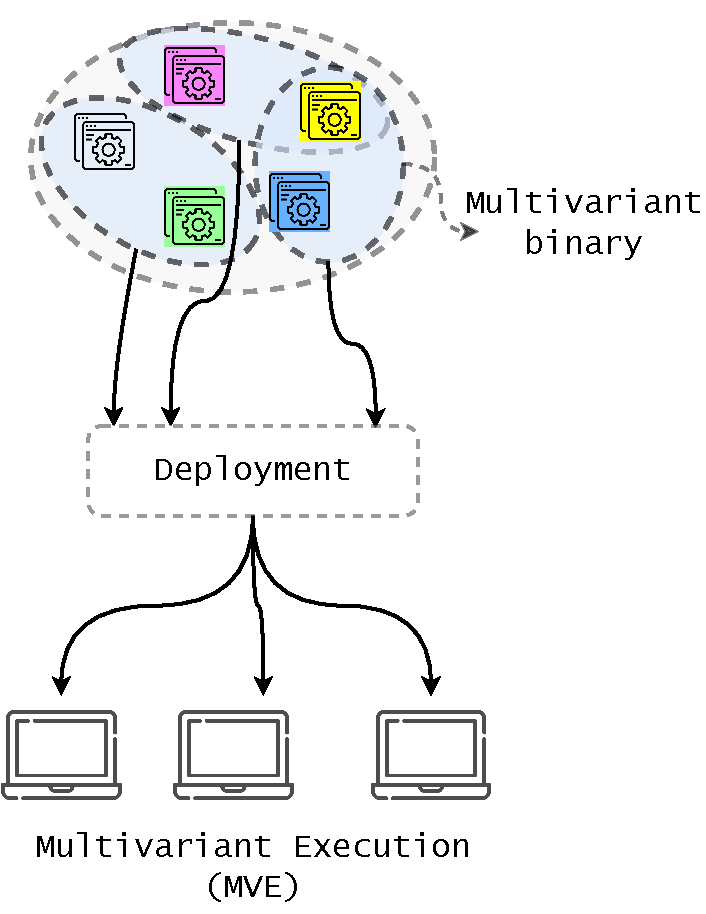
\includegraphics[height=2.8in]{diagrams/mve.pdf}
        \caption{Multivariant Execution scenario. Given a pool of program variants, a sample of the pool is packaged in a multivariant binary that is deployed per. Each deployment randomly selects which multivariant binary is assigned to each host. A variant from the multivariant binary is randomly executed at runtime in the host, .}        \label{diagrams:sota:mve}

    \end{subfigure}
    \caption{Software Diversification usages. }
\end{figure}



\begin{usage}{Randomization:}
    \label{usage:randomization}
    \normalfont
    In the first scenario, a program is selected from the collection of variants (program's variant pool) and at each deployment it is assigned to a random client. This strategy prevents the usage of one variant to exploit another clients. When clients run two program variants, a potential attacker must create one attack for each variant. Therefore, the attacker must spend more time and effort to get the same return on reward for an attack. Jackson \etal \cite{jackson} call this a herd inmunity, in their work they demonstrated that this usage can prevent against ROP and JIT-ROP attacks \citationneeded. Similarly, Amarilli \etal~\cite{amarilli2011can} drastically increase the number of execution traces required by a side-channel attack
    %To illustrate the impact of this usage, the Polyverse company \footnote{\url{https://polyverse.com/}} is able to provide unique Linux distributions to each one of their clients. 

    
    
\end{usage}

\begin{usage}{Multivariant Execution(MVE):}
    \label{usage:mve}
    \normalfont
    In the second scenario, multiple program variants are composed in one single binary (multivariant binary) that is randomly deployed to a client. Once in the client, the multivariant binary executes program variants during runtime, either in parallel to check for inconsistencies or a single program to randomize execution paths \cite{bhatkar03}.
    In 2006, security researchers at the University of Virginia laid the foundations of a novel approach to security that consists in executing multiple variants of the same program, \cite{cox06}. Bruschi et al. \cite{bruschi2007diversified} extended the idea of executing the variants in parallel. Simultaneously, Salamat \etal \cite{salamat2007stopping} created a C compiler and modified a standard library that generates 32-bit Intel variants where the stack grows in the opposite direction. Their approach prevents against memory corruption. 
    
    %Also, this system can be reached dynamically, like the work of Courouss{\'e} \etal, creating an MVE through code polymorphism \cite{10.1145/3281662}.  
    Notably, neatly exploiting the limit case of executing only two variants \cite{salamat2009orchestra, maurer2012tachyon,Kim2015, lu2018stopping} provides security. Davi \etal proposed Isomeron \cite{davi2015isomeron}, an approach  for execution-path randomization. Isomeron simultaneously loads the original program and a variant. While the program is running, Isomeron continuously flips a coin to decide which copy of the program should be executed next at the level of function calls. With this strategy, a potential attacker cannot predict whether the original or the variant of a program will execute.
    Agosta \etal~\cite{agosta2015meet} and Crane \etal~\cite{crane2015thwarting} used their generated programs to compile multiple functionally equivalent variants, randomizing software control flow at runtime to tackle power side-channels.  
    %Besides, . 
    

    %. Subsequent techniques focus on Multivariant. Execution for mitigating memory vulnerabilities \cite{lu2018stopping} and other specific security problems incl. return-oriented programming attacks \cite{volckaert2015cloning} and code injection \cite{SalamatJWWF11}. 
    
    %
\end{usage}


%\begin{usage}{Moving Target Defense(MTD):}
%    \label{usage:mtd}
%    \normalfont
%\autoref{usage:randomization} and \autoref{usage:mve} can be categorized as Moving Target Defense strategies. Moving Target Defense for software was first proposed as a collection of techniques that aim to improve the security of a system by constantly moving its vulnerable components \cite{MTDNationalCyberLaep, okhravi2013survey}. Usually, MTD techniques revolve around changing system inputs and configurations to reduce attack surfaces. 
%This increases uncertainty for attackers and makes their attacks more difficult. Ultimately, potential attackers cannot hit what they cannot see. 
%MTD can be implemented in different ways, including via dynamic runtime platforms \cite{10.1145/3318216.3363338}. 
%In the case of \autoref{usage:n-version}, this usage lacks of the time dimension, \ie program variants are not changed from time to time. 

%\end{usage}




\section{Statement of Novelty}
\label{sota:novelty}

We contribute to Software Diversification for \wasm using Artificial Diversification, for Randomization and Multivariant Execution usages (\autoref{usage:randomization}, \autoref{usage:mve}). 
In \autoref{table:sota:comparison} we listed related work on Artificial Software Diversification that support our work. The table is composed by the authors and the reference to their work, followed by one column for each strategy and usage ( \autoref{strategy:S1},  \autoref{strategy:S2},  \autoref{strategy:S3},  \autoref{strategy:S4},  \autoref{strategy:S5}, \autoref{usage:randomization} and \autoref{usage:mve}). The last column of the table summarize their technical contribution. Each cell in the table contains a checkmark if the strategy or the usage of the work match the previously mentioned classifications. The rows are sorted by the year of the work in ascending order. The last two rows locate our contributions. 

{
    \renewcommand{\arraystretch}{1.6}
    \newcolumntype{M}{>{\begin{varwidth}{3cm}}l<{\end{varwidth}}} %M is for Maximal column
    \begin{table}[h]
        %\small
        %\begin{sidewaystable}
        \centering
    %\setlength\minrowclearance{1.0pt}
    \resizebox{\textwidth}{!}{

        %\begin{adjustbox}{angle=90}
                \begin{tabular}[t]{ l |lllll|ll|p{6cm}|}
\textbf{Authors} & \textbf{\autoref{strategy:S1}} & \textbf{\autoref{strategy:S2}} & \textbf{\autoref{strategy:S3}} & \textbf{\autoref{strategy:S4}} & \textbf{\autoref{strategy:S5}} & \textbf{\autoref{usage:randomization}} & \textbf{\autoref{usage:mve}} & \textbf{Main technical contribution} \\
\hline\hline
Pettis and Hansen \cite{pettisochhansen} & &\checkmark & &\checkmark & &\checkmark & &Custom Pascal compiler for PA-RISC architecture \\
Chew and Song \cite{Chew02mitigatingbuffer} & & &\checkmark & & &\checkmark & &Linux Kernel recompilation. \\
Kc \etal  \cite{Kc03} & & & & &\checkmark & & &Linux Kernel recompilation. \\
Barrantes \etal  \cite{barrantes2003randomized} & & & & &\checkmark &\checkmark & &x86 to x86 transformations using Valgrind \\
Bhatkar \etal \cite{bhatkar03} &\checkmark &\checkmark & &\checkmark & &\checkmark & &ELF binary transformations \\
El-Khalil and Keromytis  \cite{ElKhalil2004} & & & & & &\checkmark & &custom GCC compiler for x86 architecture \\
Bhatkar \etal \cite{bhatkar2005efficient} &\checkmark &\checkmark & &\checkmark & &\checkmark & &C/C++ source to source transformations and ELF binary transformations \\
Younan \etal  \cite{Younan2006} & & & &\checkmark & & & &custom GCC compiler \\
Bruschi \etal \cite{bruschi2007diversified} & & & &\checkmark & &\checkmark & &ELF binary transformations. \\
Salamat \etal \cite{salamat2007stopping} & & &\checkmark & & & &\checkmark &Custom GNU compiler \\
Jacob \etal \cite{jacob2008superdiversifier} &\checkmark &\checkmark & & & & & &x86 to x86 transformations \\
Salamat \etal \cite{salamat2009orchestra} & & & &\checkmark & & &\checkmark &x86 to x86 transformations \\
Amarilli \etal  \cite{amarilli2011can} &\checkmark & & & &\checkmark &\checkmark & &Polymorphic code generator for ARM architecture \\
Jackson  \cite{jackson} &\checkmark & & & & &\checkmark &\checkmark &LLVM compiler, only backend for x86 architecture \\
Cleemput \etal  \cite{ElKhalil2004} &\checkmark & & & & &\checkmark & &x86 to x86 transformations \\
Homescu \etal \cite{homescu2013profile} &\checkmark & & & & &\checkmark & &LLVM 3.1.0$^\dagger$ \\
Crane \etal  \cite{crane2015thwarting} &\checkmark &\checkmark &\checkmark & & & &\checkmark &LLVM, only backend for x86 architecture \\
Davi \etal \cite{davi2015isomeron} & & & & & & &\checkmark &Windows DLL instrumentation \\
Courouss{\'e} \etal  \cite{courousse2016runtime} &\checkmark &\checkmark & & &\checkmark & \checkmark&  &Custom GCC compiler targeting microcontrollers \\
Lu \etal \cite{lu2018stopping} & & & &\checkmark & & &\checkmark &GNU assembler for Linux kernel \\
Belleville \etal \cite{10.1145/3281662} &\checkmark & & &\checkmark & &\checkmark & &Only C language frontend, LLVM 3.8.0$^\dagger$ \\
Aga \etal \cite{aga2019smokestack} & & & &\checkmark & &\checkmark & &Data layout randomization, LLVM 3.9$^\dagger$ \\
{\"O}sterlund \etal \cite{osterlund2019kmvx} & & & &\checkmark & & &\checkmark &Linux Kernel recompilation. \\
Xu \etal \cite{xu2020merr} & & & &\checkmark & &\checkmark & &Custom kernel module in Linux OS \\
Lee \etal \cite{lee2021savior} & & & &\checkmark & &\checkmark & &LLVM 12.0.0 backend for x86 \\
Romano \etal \cite{wobfuscator} & & & \checkmark & & &\checkmark & & JavaScript and Wasm intermixing \\

%\hline
%\hline
%Cabrera Arteaga \etal \cite{CROW} &\checkmark &\checkmark &\checkmark &\checkmark & &\checkmark & &Any frontend language for LLVM version 12.0.0 targeting Wasm  backend \\
%Cabrera Arteaga \etal \cite{MEWE} &\checkmark &\checkmark &\checkmark &\checkmark & & &\checkmark &Any frontend and backend language for LLVM version 12.0.0 \\

\end{tabular}
        %\end{adjustbox}
    }

        {
            \scriptsize
            $^\dagger$ Notice that LLVM only supports \wasm backend from version 8.0.0
        }

        \caption{The first and second columns in the table correspond to the author names and the references to their work, followed by one column for each strategy and usage ( \autoref{strategy:S1},  \autoref{strategy:S2},  \autoref{strategy:S3},  \autoref{strategy:S4},  \autoref{strategy:S5}, \autoref{usage:randomization} and \autoref{usage:mve}). The last column of the table summarizes the technical contribution and the reach of the referred work. Each cell in the table contains a checkmark if the strategy or the usage of the work match the previously mentioned classifications. The rows are sorted by the year of the work in ascending order. The last two rows locate our contributions. }
        \label{table:sota:comparison}
\end{table}
        %\end{sidewaystable}
}

% Move to introduction
%The primary motivation for our contributions is that we see in \wasm a monoculture problem. If one environment is vulnerable, all the others are vulnerable in the same manner as the same \wasm binary is replicated. 
%Besides, the \wasm environment lacks natural diversity \cite{natural_diversity}. Compared to the work of Harrand \etal \citationneeded, in WebAssembly, one could not use preexisting and different program versions to provide diversification. On the other hand, while the number of related work for software diversity is large, only one approach has been applied to the context of \wasm. 
% Move to the table
%To the best of our knowledge, the closest diversification work on the browsers involving \wasm is the work of Romano \etal \cite{wobfuscator}. They proposed to de-inline JavaScript subexpressions and replace them with function calls to \wasm counterparts.  They empirically demonstrated that malware classifiers could be evaded with this diversification technique. 
\wasm is a novel technology, and the adoption of defenses for it is still under development \cite{Narayan2021Swivel, johnson2021}. The current limitations on security and the lack of preexisting diversity motivate our work on software diversification as one preemptive mitigation among a wide range of security countermeasures.
% CROW
Our first contribution, CROW \cite{CROW} generates multiple program variants for \wasm using the LLVM pipeline.
It contributes to state of the art in artificially creating randomization for \wasm (\autoref{usage:randomization}). Because of the specificities of code execution in the browser (mentioned in \autoref{sota:wasm}), this can be considered a randomization approach. For example, since \wasm is served at each page refreshment, every time a user asks for a \wasm binary, she can be served a different variant provided by CROW. 
% Move to intro
%Besides, our contribution can be used in fuzzing campaigns \citationneeded to provide reliability. The diversification created by CROW can unleash hidden behaviors in compilers and interpreters. Thanks to CROW, a bug was discovered in the Lucet compiler \footnote{\url{https://www.fastly.com/blog/defense-in-depth-stopping-a-wasm-compiler-bug-before-it-became-a-problem}}.
%MEWE
With MEWE \cite{MEWE}, our second contribution, we randomly select from several variants at runtime (\autoref{usage:mve}), creating a multivariant execution scheme that randomizes the observable behaviors at each run of the program. Notably, researching on MVE in a distributed setting like the Edge \citationneeded has been less researched. We use the natural redundancy of Edge-Cloud computing architectures to deploy an internet-based MVE.

% Move to intro
% Only Voulimeneas \etal recently proposed a multivariant execution system by parallelizing the execution of the variants in different machines \cite{voulimeneas2021dmvx} for the sake of efficiency. 
% Move this to the technical part
%CROW, extrapolates the idea of superdiversification \cite{jacob2008superdiversifier} for \wasm. CROW works directly with LLVM IR, enabling it to generalize to more languages and CPU architectures, something not possible with the x86-specific approach of previous works.

%CROW focuses on the static diversification of software. However, 





\subsection*{Conclusions}
In this chapter, we presented the background on the \wasm language, including its security issues and related work.
This chapter aims to settle down the foundation to study automatic diversification for \wasm. 
We highlighted related work on Artificial Software Diversification, showing that it has been widely researched, not being the case for \wasm. 
On the other hand, current available implementations for Software Diversification cannot be directly ported to Wasm. 
The current limitations on security and the lack of software diversity approaches for \wasm motivate our work.
We place our contributions in the field of artificial diversity. 
In \autoref{chapter:technical} we describe the technical details that lead our contributions. 
Besides, the impact of our contributions is evaluated by following the methodology described in \autoref{chapter:method}.
